\clearpage
\subsection{Boolean Data} % (fold)
\label{sub:boolean_data}

The Boolean\footnote{Named after George Bool's Boolean logic.} Data Type is a \nameref{sub:type} used to represent \textbf{truth}. A Boolean value will either be \textbf{true} or \textbf{false}. These values are used extensively in the control flow statements to determine the action to perform.

\begin{figure}[h]
   \centering
   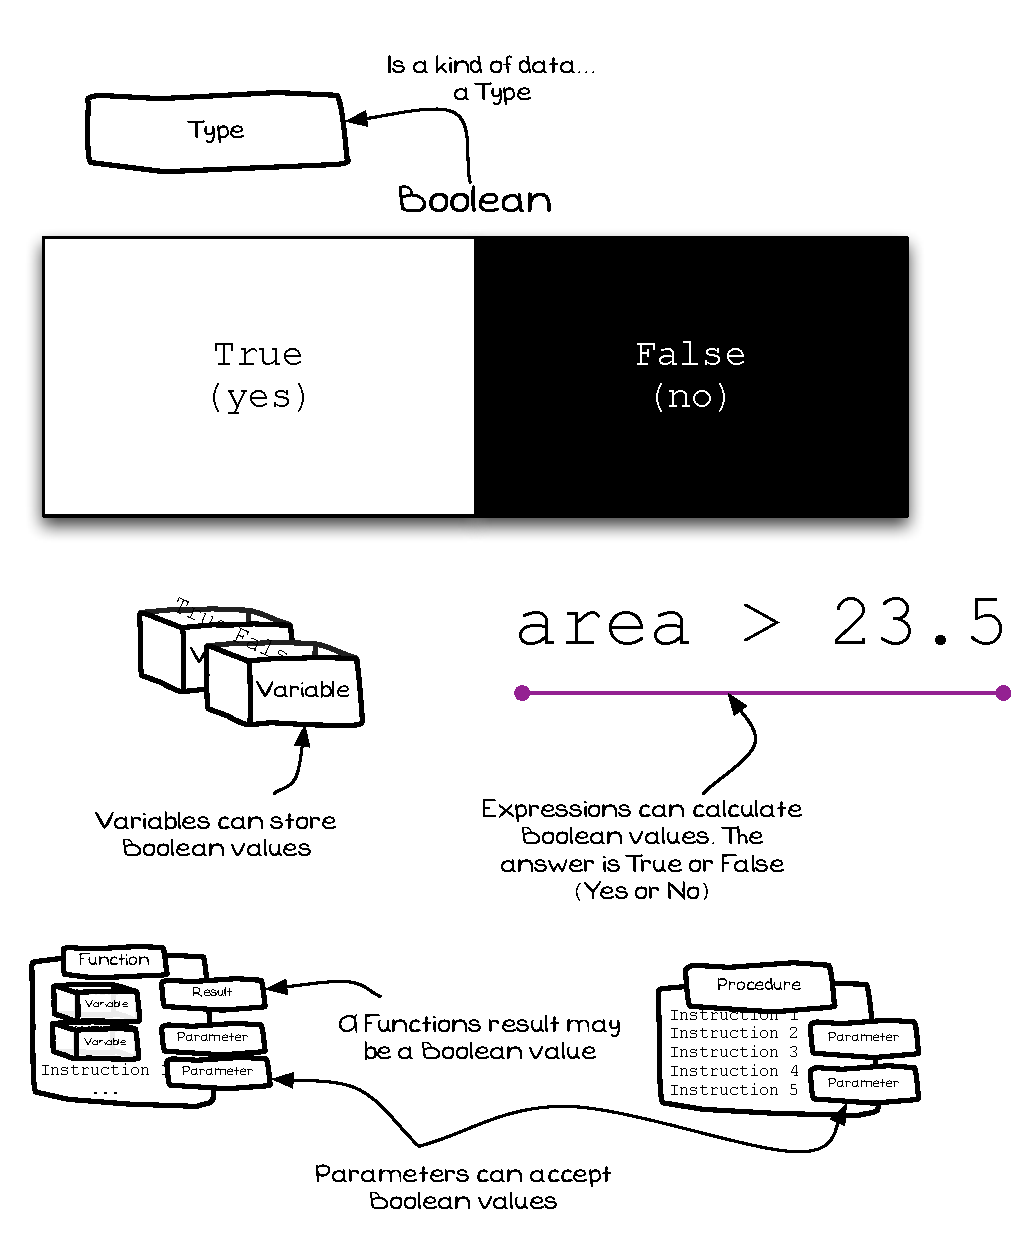
\includegraphics[width=0.8\textwidth]{./topics/control-flow/diagrams/BooleanData} 
   \caption{Boolean data represents truth}
   \label{fig:boolean-data}
\end{figure}

\mynote{
\begin{itemize}
  \item Boolean is an existing \textbf{artefact}, it is a \nameref{sub:type} that has been defined to represent truth values.
  \item A Boolean value is either \textbf{true} or \textbf{false}. You can also think of these as \emph{yes} and \emph{no}.
  \item Boolean values are used in most of the control flow statements.
  \item The Boolean type can be used in the same way as other types.
\end{itemize}
}
% subsection boolean_data (end)

\clearpage
\subsubsection{Comparisons} % (fold)
\label{sub:comparisons}

Comparisons are a common way of getting Boolean values in your code. These \nameref{sub:expression}s allow you to compare two values to check for a given condition. For example, the Expression shown in Figure \ref{fig:boolean-data} is asking if the \emph{value} in the \texttt{area} variable is larger than \texttt{23.5}. The result of this expression will be either \texttt{true} or \texttt{false} depending on the current value stored in \texttt{area}. Table \ref{tbl:bool-expr-sample} lists some example values for this expression, given different values stored in the \texttt{area} variable.

\begin{table}[h]
  \centering
  \begin{tabular}{|c|c|}
    \hline
    \textbf{Value in \texttt{area}} & \textbf{\texttt{area > 23.5}} \\
    \hline
    \texttt{73.2} & \texttt{true} \\
    \hline
    \texttt{-2.5} & \texttt{false} \\
    \hline
    \texttt{23.5} & \texttt{false} \\
    \hline
  \end{tabular}
  \caption{Example values for the expression \texttt{area > 23.5}}
  \label{tbl:bool-expr-sample}
\end{table}

Programming languages offer a range of different comparison operators. These typically include comparisons to check if values are the same or different, and to check if one value is larger or small than another. The different operators for C and Pascal are listed in Table \ref{tbl:comparisons}.

\begin{table}[h]
  \centering
  \begin{tabular}{|c|c|c|c|}
    \hline
     & \textbf{Description} & \textbf{C} & \textbf{Pascal} \\
    \hline
    \textbf{Equal} & Are the values the same? & \texttt{a == b} & \texttt{a = b} \\
    \hline
    \textbf{Not Equal} & Are the values different? & \texttt{a != b} & \texttt{a <> b} \\
    \hline
    \textbf{Larger Than} & Is the left value larger than the right? & \multicolumn{2}{c|}{\texttt{a > b}}  \\
    \hline
    \textbf{Less Than} & Is the left value smaller than the right? & \multicolumn{2}{c|}{\texttt{a < b}}  \\
    \hline
    \textbf{Larger Or Equal} & Is the left value equal or larger than the right? & \multicolumn{2}{c|}{\texttt{a >= b}}  \\
    \hline
    \textbf{Less Or Equal} & Is the left value smaller or equal to the right? & \multicolumn{2}{c|}{\texttt{a <= b}}  \\
    \hline
    
  \end{tabular}
  \caption{Comparison Operators}
  \label{tbl:comparisons}
\end{table}

\mynote{
\begin{itemize}
  \item Comparisons can only be performed between \textbf{two} values.
  \item The values on either side of the comparison are \nameref{sub:expression}s, allowing you to calculate the values being compared.
\end{itemize}
}

\csection{
C uses a double equal (\texttt{==}) for comparison as the single equals (\texttt{=}) is used for assignment.
}

% subsection comparisons (end)

\clearpage
\subsubsection{Logical Operators} % (fold)
\label{sub:logical_operators}

The comparison operators allow you to compare \emph{two} values. This is very useful, but in itself is incomplete. What, for example, do you do when you want to compare three or more values? While you are limited to two values with the comparison operators, there are other operators that allow you to \textbf{combine} Boolean expressions. This will enable you to combine together multiple Boolean values into a single Expression.

There are four main \emph{logical operators}: \textbf{and}, \textbf{or}, \textbf{xor}, and \textbf{not}. Each of these operators works on two Boolean values, combining them to give a new Boolean value. For example, the \emph{and} operator allows you to check if \emph{both} of the expressions are true. The expression \texttt{area > 0 and area < 10} will be true only when area is both larger than zero and less then ten.

\begin{figure}[h]
   \centering
   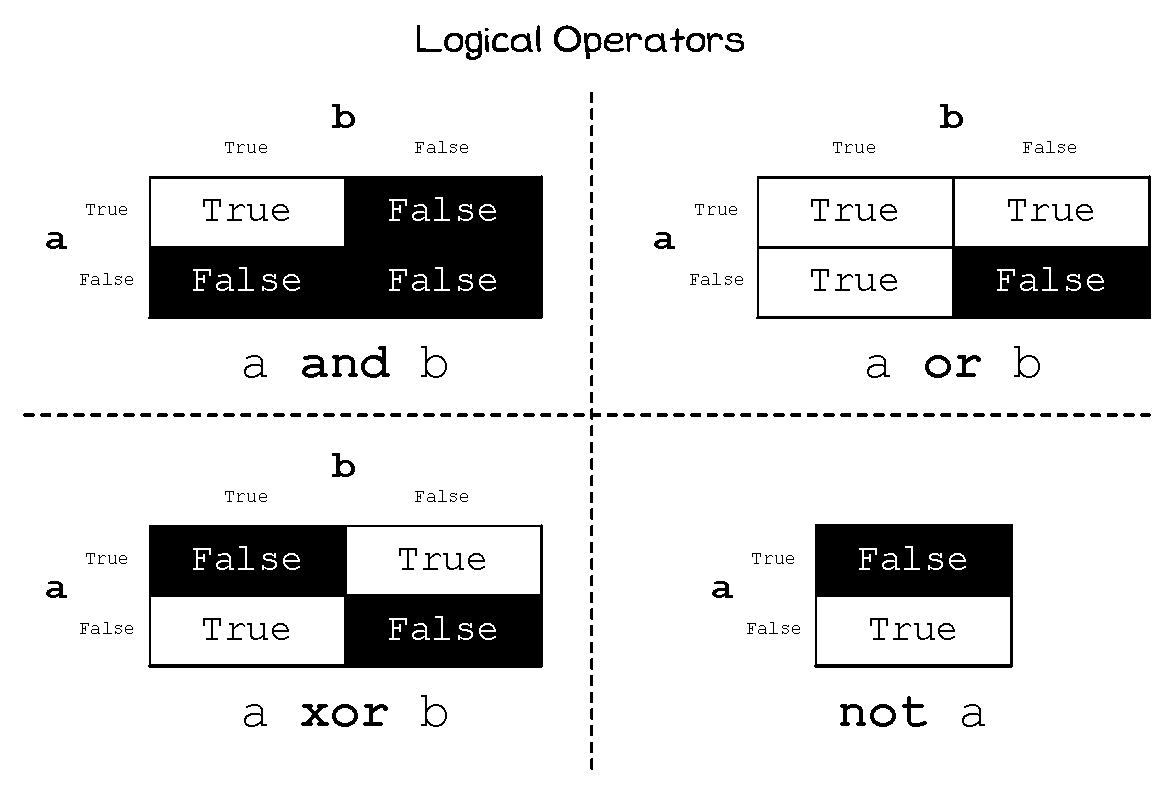
\includegraphics[width=0.7\textwidth]{./topics/control-flow/diagrams/LogicalOperators} 
   \caption{Logical Operators combine Boolean values}
   \label{fig:logical-operators}
\end{figure}

\begin{table}[h]
  \centering
  \begin{tabular}{|c|c|c|c|}
    \hline
     & \textbf{Description} & \textbf{C} & \textbf{Pascal} \\
    \hline
    \textbf{And} & Are both values True? & \texttt{a \&\& b} & \texttt{a and b} \\
    \hline
    \textbf{Or} & Is at least one value True? & \texttt{a || b} & \texttt{a or b} \\
    \hline
    \textbf{Xor} & Is one value True, and the other False? & \texttt{a \^{} b} & \texttt{a xor b} \\
    \hline
    \textbf{Not} & Is the value False? & \texttt{!a} & \texttt{not a}  \\
    \hline
  \end{tabular}
  \caption{Logical Operators}
  \label{tbl:logical-operators}
\end{table}

\begin{table}[h]
  \centering
  \begin{tabular}{|c|c|c|c|c|c|}
    \hline
    \multirow{2}{*}{area }& \multirow{2}{*}{\texttt{area > 0}} & \multirow{2}{*}{\texttt{area < 10}} & \multicolumn{3}{c|}{\texttt{area > 0 {\textbf{\ldots}} area < 10}} \\
    \cline{4-6}
     &  &  & \textbf{and} & \textbf{or} & \textbf{xor} \\
    \hline
    \texttt{\textbf{5}} & True & True & True & True & False \\
    \hline
    \texttt{\textbf{27}} & True & False & False & True & True \\
    \hline
    \texttt{\textbf{0}} & False & True & False & True & True \\
    \hline
  \end{tabular}
  \caption{Example Logical Expressions}
  \label{tbl:example_logical_expr}
\end{table}

\mynote{
\begin{itemize}
  \item Table \ref{tbl:example_logical_expr} has some example expressions.
  \item The tables in Figure \ref{fig:logical-operators} show the values of the different logical operators. These are known as \textbf{Truth Tables}.
  \item Table \ref{tbl:logical-operators} outlines the different logical operators, and how they are coded in C and Pascal.
\end{itemize}
}



% subsection boolean_logic (end)